\documentclass[a4paper,11pt,fleqn]{article}%fleqn pour aligner les equations à gauche
\usepackage{graphicx}
\usepackage[utf8]{inputenc}  
\usepackage[T1]{fontenc}
\usepackage{lscape}

\usepackage{tgheros,textcomp}%Police Arial
\renewcommand{\familydefault}{\sfdefault}

%\setlength{\mathindent}{0pt}%indentation dans math = 0

\usepackage[top = 1cm, bottom = 2cm, left = 1cm, right = 1cm]{geometry}
\usepackage{titlesec}
%\setcounter{secnumdepth}{4}
\usepackage{xcolor}
\usepackage{amssymb} %double flèche de réaction
\usepackage{mathrsfs}%farraday
\usepackage{xtab}%tableau sur plusieurs pages
\usepackage{esvect}%grands vecteurs

\usepackage[version=4]{mhchem} %equations chimiques

\usepackage{array}
\usepackage{chemfig}
\usepackage{multirow}
%\usepackage{sectsty}

\usepackage{caption}
\usepackage{adjustbox}
\usepackage[labelformat=simple]{subfig}
\usepackage{float}


\usepackage{amsmath}
\usepackage{amssymb}
\usepackage[cal=boondoxo]{mathalfa} 
\usepackage{enumitem}
\usepackage{lastpage}
\usepackage{tcolorbox}
\usepackage{siunitx}
\usepackage[european, straightvoltages, RPvoltages]{circuitikz}
\usepackage{tikz}
\usetikzlibrary{shapes.geometric}
\usetikzlibrary{calc}
\usetikzlibrary{automata,positioning}
\usepackage{multicol}
\usepackage{eqnarray}
\usepackage{tabularx,colortbl}%colorer fond cellules

\sisetup{
	detect-all,
	output-decimal-marker={,},
	group-minimum-digits = 3,
	group-separator={~},
	number-unit-separator={~},
	inter-unit-product={~}
} %setup pour SIunitx

\usepackage{listings}%pour insérer le code python
\definecolor{codegreen}{rgb}{0,0.6,0}
\definecolor{codegray}{rgb}{0.5,0.5,0.5}
\definecolor{codepurple}{rgb}{0.58,0,0.82}
\definecolor{backcolour}{rgb}{0.95,0.95,0.92}


\titleformat{\section}
{
\vspace{.8ex}%
\normalfont \bfseries \large}
{\thesection.}{.5em}{\bfseries}

\renewcommand{\thesection}{\arabic{section}}
\titlespacing{\section}{0pt}{1em}{.5em}
\renewcommand{\thesubsection}{\hspace{1cm}\alph{subsection}.}
\renewcommand\thesubfigure{\textbf{Document \arabic{subfigure} :}}

\title{\vspace{-1cm}\large 
	\begin{tabular}{|>{\centering}m{5cm}|>{\centering}m{8cm}|>{\centering\arraybackslash}m{4cm}|}
		\hline
		Cours & \textbf{\textsc{La Radioactivité}} &  Chapitre 8 \\
		\hline
\end{tabular}}
\date{}

\newpagestyle{mystyle}{%
	\setfoot{ROSALIE}{\thepage\,$|$\,\pageref{LastPage}}{}
}
\renewpagestyle{plain}{%
	\setfoot{ROSALIE}{\thepage\,$|$\,\pageref{LastPage}}{}
}

\pagestyle{mystyle}

\newenvironment{itemize*}%
{\begin{itemize}[label=$-$,labelindent=0pt, leftmargin=*,topsep=0pt]%
		\setlength{\itemsep}{0pt}%
		\setlength{\parskip}{0pt}}%
	{\end{itemize}}

\newenvironment{itemize**}%
{\begin{itemize}[label=,labelindent=0pt, leftmargin=*,topsep=0pt]%
		\setlength{\itemsep}{0pt}%
		\setlength{\parskip}{0pt}}%
	{\end{itemize}}

\renewcommand{\arraystretch}{1.5}

\begin{document}
	\maketitle
	\vspace{-3cm}
\section{Désintégration radioactive}
	\subsection{Stabilité et instabilité des noyaux}
	118 éléments chimiques sont connus à ce jour. Ces éléments présentent un grand nombre d'\textbf{isotopes} : certains sont stables ou quasi-stables (environ 300) mais la grande majorité d'entre eux sont \textbf{instables} et considérés comme \textbf{radioactifs} (environ 3000).\\
	L'ensemble des noyaux connus sont répertoriés dans un \textbf{diagramme (N,Z)} où N représente le nombre de neutrons et Z le nombre de protons. Les noyaux stables figurent dans une zone centrale, appelée vallée de la stabilité. Les noyaux instables figurent de part et d'autre de cette vallée. Leur proportion de neutrons et de protons ne permet pas d'assurer leur cohésion.
	\begin{center}
		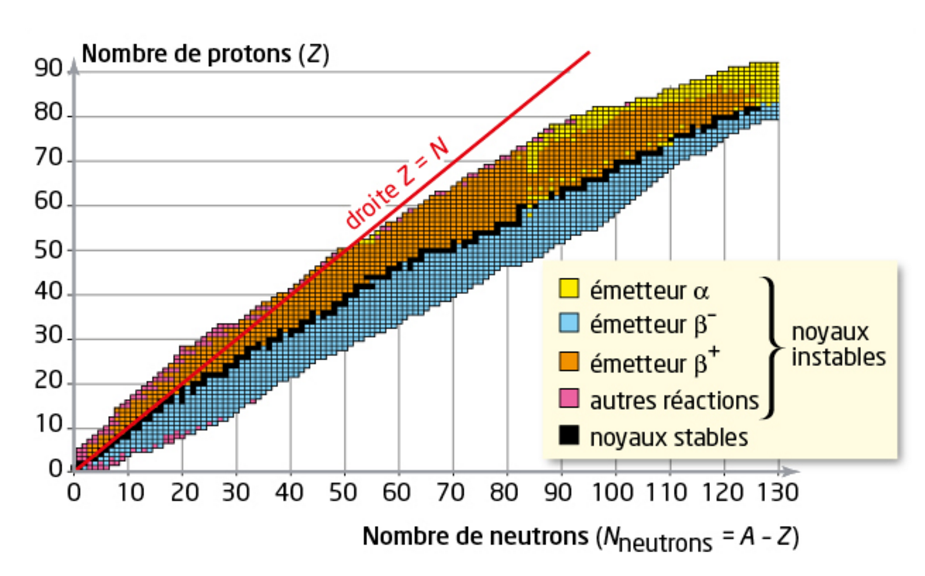
\includegraphics[scale=.5]{Ressources/TSPE_C15_Cours_Fig8.png}
	\end{center}
	
	
	\subsection{Différents types de radioactivité}
	Afin de se stabiliser, un noyau instable se désintègre \textbf{naturellement} et \textbf{spontanément} en un nouveau noyau d'un autre élément chimique. cette désintégration s'accompagne de l'\textbf{émission d'une particule} et d'un \textbf{rayonnement} $\gamma$ (gamma). C'est ce rayonnement qui est à l'origine du nom "radioactivité".\\
	On distingue différents types de radioactivité, selon le type de particule émise :
	\begin{itemize}
		\item \begin{tabular}{m{.6\textwidth}m{.4\textwidth}}
			La radioactivité $\alpha$ correspond à l'émission d'une \textbf{particule} $\alpha$ (noyau d'hélium) selon la réaction d'équation :&\multirow{3}{*}{
		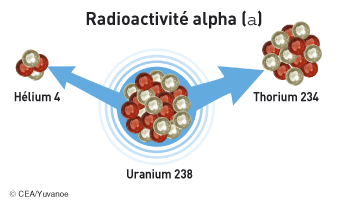
\includegraphics[scale=.7]{Ressources/TSPE_C15_Cours_Fig1.png}}\\
		\textcolor{gray}{Exemple :} \ce{^{238}_{92}U -> ^{234}_{90}Th + ^{4}_{2}He}&\\
		Elle concerne les noyaux lourds (grand nombre de nucléons).&\\		
		\end{tabular}
		
		\item \begin{tabular}{m{.6\textwidth}m{.4\textwidth}}
			La radioactivité $\beta -$ correspond à l'émission d'un \textbf{électron} et d'un anti-neutrino selon la réaction d'équation :&\multirow{3}{*}{
		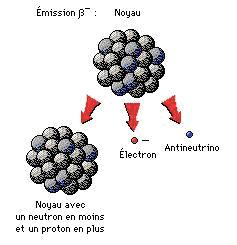
\includegraphics[scale=.7]{Ressources/TSPE_C15_Cours_Fig2.png}}\\
		\textcolor{gray}{Exemple :} \ce{^{14}_{6}C -> ^{14}_{7}N + ^{0}_{-1}e + ^0_0$\bar{\nu_e}$}&\\
		Elle concerne les noyaux possédant un excès de neutrons.&\\
		\end{tabular}
		
		\item  \begin{tabular}{m{.6\textwidth}m{.4\textwidth}}
		La radioactivité $\beta +$ correspond à l'émission d'un \textbf{positon} et d'un neutrino selon la réaction d'équation :&\multirow{3}{*}{
		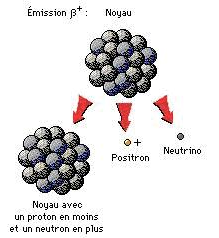
\includegraphics[scale=.7]{Ressources/TSPE_C15_Cours_Fig3.png}}\\
		\textcolor{gray}{Exemple :} \ce{^{30}_{15}P -> ^{30}_{14}Si + ^{0}_{1}e + ^0_0\nu_e}&\\
		Elle concerne les noyaux possédant un excès de protons.&\\
		\end{tabular}
	\end{itemize}
	
\vspace{2cm}
Le type de radioactivité selon lequel un noyau va de désintégrer peut se repérer dans le diagramme (N,Z). Quel que soit le type de désintégration, il y aura \textbf{conservation du nombre de charges électriques Z et du nombre de masse A}.\\
Par ailleurs, la plupart des noyaux fils issus d'une désintégration radioactive sont dans un \textbf{état excité} (noté \ce{^A_ZX^$*$}). Ils retrouvent leur état fondamental en émettant un photon de haute énergie (\textbf{photon} $\gamma$) :\\
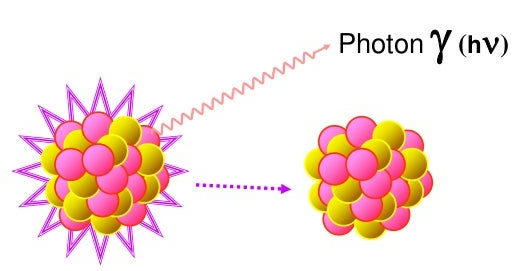
\includegraphics[scale=.5]{Ressources/TSPE_C15_Cours_Fig3b.png}

\section{Décroissance radioactive}
	\subsection{Aléatoire ou prévisible}
	La désintégration d'\textbf{un} noyau radioactif est un phénomène \textbf{spontané}, \textbf{inéluctable} et \textbf{aléatoire}. Il n'est donc pas possible de savoir à l'avance si un noyau radioactif se sera désintégré à un instant $t$ donné.\\
	En revanche, lorsque le nombre de noyaux radioactifs est suffisamment grand, il est possible de prévoir combien de noyaux se seront désintégrés à un instant $t$ en raisonnant à l'aide de probabilités. Cela permet de suivre l'évolution du nombre de noyaux radioactifs désintégrés (ou du nombre de noyaux radioactifs restant, c'est à dire non désintégrés).
	
	\subsection{Activité radioactive}
		\subsubsection*{Définition}
		Soit $N$ le nombre de noyaux radioactifs d'un échantillon. on appelle \textbf{activité A} le nombre moyen de désintégration par seconde survenant dans un échantillon de noyaux radioactifs. Ainsi : 
		$$A = \dfrac{\text{nb de désintégrations}}{\Delta t} = \dfrac{N(t)-N(t+\Delta t)}{\Delta t} = \dfrac{-\Delta N}{\Delta t}$$
	Pour une durée infiniment faible :
		$$\mathbf{A = \dfrac{-dN}{dt}}$$
		
		\subsubsection*{Unité}
		L'activité $A$ s'exprime en Becquerel (\unit{\becquerel}) en hommage ua physicien éponyme, découvreur de la radioactivité en 1896. \SI{1}{Bq} = 1 désintégration par seconde.\\
		\begin{tabular}{|c|c|c|c|c|}
			\hline \textbf{Source} & Eau douce (1L) & Légumes (1kg) & Corps humain (70kg)& Uranium 238 (1g)\\
			\hline \textbf{Activité (en \unit{\becquerel})} & 1 & 150 & 8000 & 12000\\
			\hline
		\end{tabular}\\
		
		Remarque : l'activité $A$ en Becquerel mesure le niveau de radioactivité d'un échantillon, par sa dangerosité (même si il y a un lien entre les deux !)\\
		\begin{tabular}{|>{\centering}m{6cm}|>{\centering}m{6cm}|>{\centering\arraybackslash}m{6cm}|}
			\hline \multicolumn{3}{|c|}{\textbf{Les unités de mesure de la radioactivité}}\\
			\hline
			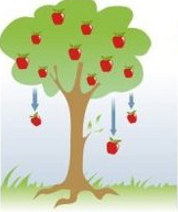
\includegraphics[scale=.5]{Ressources/TSPE_C15_Cours_Fig4a.png}&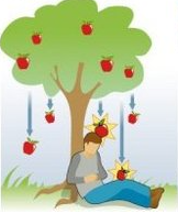
\includegraphics[scale=.5]{Ressources/TSPE_C15_Cours_Fig4b.png}&
\includegraphics[scale=.5]{Ressources/TSPE_C15_Cours_Fig4c.png} \rule[3cm]{0cm}{0cm}\\
			Le nombre de pommes qui tombent peut se comparer au \textbf{Becquerel}. (nombre de désintégrations par seconde) & Le nombre de pommes reçues par le dormeur peut se comparer au \textbf{Gray} (dose absorbée) & L'effet laissé sur le corps peut se comparer au \textbf{Sievert}. (\textbf{effet biologique}, fonction du type de radiation, de l'organisme concerné et du temps d'exposition)\\
			\hline
		\end{tabular}\\
		
		\subsubsection*{Relation}
		\noindent \begin{minipage}{.65\linewidth}
			Au fur et à mesure des désintégrations, il reste de moins en moins de noyaux radioactifs dans l'échantillon, donc de moins en moins de désintégrations surviennent chaque seconde. Ainsi, l'activité diminue à mesure que le nombre de noyaux radioactifs diminue.\\
			Plus précisément, l'activité est proportionnelle au nombre de noyaux radioactifs de l'échantillon :
			$$\mathbf{A(t)=\lambda \times N(t)}$$
			$\lambda$ est appelée \textbf{constante radioactive} (en \unit{\per\second}), elle dépend du type de noyau radioactif et correspond à la probabilité de désintégration par unité de temps.
		\end{minipage}
		\begin{minipage}{.35\linewidth}
			\centering
			\begin{tabular}{|c|>{\centering\arraybackslash} m{4cm}|}
				\hline 
				\textbf{Noyau}&\textbf{Constante radioactive $\lambda$} (en \unit{\per\second})\\
				\hline \ce{^218_86Rn} & \num{19,5}\\
				\hline \ce{^220_86Rn} & \num{1,25E-2}\\
				\hline \ce{^222_86Rn} & \num{2,10E-6}\\
				\hline \ce{^222_90Th} & \num{310}\\
				\hline \ce{^232_90Th} & \num{1,56E-18}\\
				\hline
			\end{tabular}
		\end{minipage}

	\subsection{Loi de décroissance  radioactive}
		\subsubsection*{Raisonnement à connaître :}
		Comme :
		$$ A=\dfrac{-dN}{dt}\text{ et }A(t) = \lambda \cdot N(t) $$
		Alors : $$\dfrac{-dN}{dt} = \lambda \cdot N(t)$$
		Soit : $$\dfrac{dN}{dt} + \lambda \cdot N(t)=0$$
		La solution générale de cette équation différentielle est de la forme : $N(t)=Ke^{-\lambda t}$.
\newpage
		On détermine $K$ à l'aide des conditions initiales : \\
		$$\text{À } t=0 \text{, } N(t)=n_0$$
		$$Ke^{-\lambda \times 0} = N_0$$
		$$K = N_0$$
		Ainsi : $$\mathbf{N(t)=N_0e^{-\lambda t}}$$

		\noindent \begin{minipage}{.6\linewidth}
		Le nombre de noyaux radioactifs d'un échantillon suit une loi de décroissance exponentielle, dite \textbf{loi de décroissance radioactive}.\\
			Comme $$A(t)=\lambda N(t)\text{, alors } A(t) = \lambda N_0 e^{-\lambda t}$$
			Donc : $$A(t)=A_0e^{-\lambda t}$$
			L'activité $A$ suit également une \textbf{loi de décroissance radioactive}.
		\end{minipage}
	\begin{minipage}{.4\linewidth}
		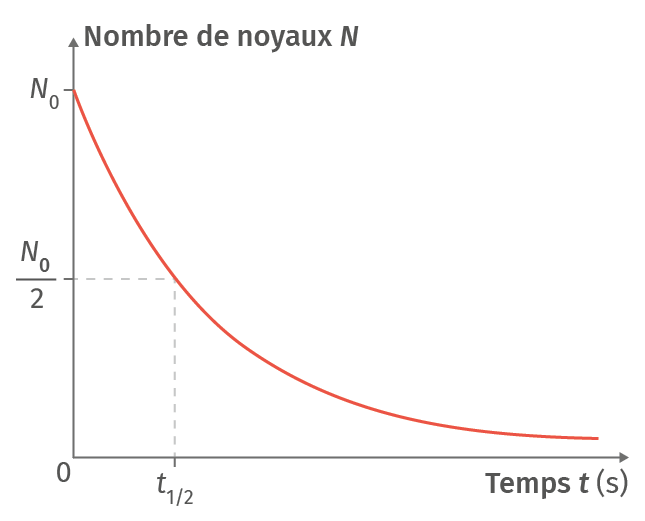
\includegraphics[scale=.5]{Ressources/TSPE_C15_Cours_Fig7.png}
	\end{minipage}
		
	\subsection{Demi-vie}
	La durée au bout de laquelle la moitié des noyaux radioactifs initialement présents se sont désintégrés est appelée \textbf{demi-vie} ($t_{1/2}$). la demi-vie est caractéristique d'un type de noyau radioactifs.\\
	\noindent \begin{minipage}{.5\linewidth}
		La demi-vie peut se déterminer graphiquement ou à l'aide de la constante radioactive :\\
		$$N(t_{1/2}) = \dfrac{N_0}{2}$$
		$$N_0e^{-\lambda t_{1/2}}=\dfrac{N_0}{2}$$
		$$e^{-\lambda t_{1/2}}= \dfrac{1}{2}$$
		$$ln(e^{-\lambda t_{1/2}})=ln(\dfrac{1}{2})$$
		$$-\lambda t_{1/2} = ln(1)-ln(2)$$
		$$\text{Or $ln(1) = 0$, donc : }$$
		$$-\lambda t_{1/2} = - ln(2)$$
		$$\mathbf{t_{1/2}=\dfrac{ln(2)}{\lambda}}$$
	\end{minipage}
	\begin{minipage}{.5\linewidth}
		Comme les constantes radioactives, les demi-vies des noyaux radioactifs prennent des valeurs très diverses.\\
		\begin{tabular}{|c|c|}
			\hline
			\textbf{Isotopes radioactifs} & \textbf{Temps de demi-vies (a)}\\
			\hline \ce{^8_4Be}&\num{2,12E-24}\\
			\hline \ce{^{131}_{53}I}&\num{2,20E-2}\\
			\hline \ce{^{60}_{27}Co}&\num{5,27}\\
			\hline \ce{^{14}_{6}C}&\num{5,73E3}\\
			\hline \ce{^{129}_{53}I}&\num{1,57E7}\\
			\hline \ce{^{232}_{90}Th}&\num{1,41E9}\\
			\hline
		\end{tabular}
	\end{minipage}
	 
\end{document}
